In multi-tenancy \textit{variability} is a key concept. The term was first introduced in the car industry, where customers could choose certain \textit{variants} of chassis, engine and color \cite[p. 153]{kabbedijk2011variability}. 
In research on software engineering the concept was defined as ``the ability of a software system or artefact to be efficiently extended, changed, customized or configured for use in a particular context'' \cite{svahnberg2005taxonomy}.
Two keywords from this definition are customization and configuration. In a multi-tenant context configuration is preferred over customization \cite{sun2008software} as customization defines the process of reengineering an application, maintaining multiple branches and deploying these branches separately, while configuration can be done at run-time and does not require multiple instances or branches.

\subsubsection{Why is variability needed}
There are several reasons why variability is needed. 
First of all based on country, segment or branch different currencies, legislation and tax rules may apply. This is especially important in financial applications. 
Secondly different customers can require different functionality properties, layout options and/or quality of service (such as privacy and performance).
% MAYBE-TODO: this paragraph could be more elaborate

\subsubsection{Levels of variability}
Variability can be accomplished on different levels. 
Dependent on the scale of the application different patterns become be relevant. Large applications often consist of \textit{components} offering a specific \textit{service} and variability can be accomplished by dynamically swapping these components for different tenants, or by activating or deactivating specific components \cite{mietzner2008defining}. 

In smaller applications and within components different patterns become relevant. For example, one can customize an application by using dependency injection \cite{walraven2011middleware} or context oriented programming \cite{truyen2012context}.

Two types of variability can be distinguished, external and internal variability \cite{mietzner2009variability}:
 \begin{itemize}
\item \textbf{External variability} is this variability that is communicated to the customers and most of the times this variability is \textbf{Customer-driven} and is implemented because customers asked for it or because the developers thought the customers would ask for it. 
\item In contrast  \textbf{internal variability} exists because of implementation details. For example some - external - variants may depend on some internal variation.
\end{itemize}

%reasons for variability [5]
%different papers describe different categorizations

\subsubsection{Variability Modeling}
For all stakeholders in a multi-tenant application it's important that a variability model exists. For the developer it's important to document all variation build in to the application to keep the application maintainable for both current and new developers. 
For SaaS providers it's important to have a model of the application to build rules for automatically deploying new instances of the application that support (many) new tenants or migrating and reconfiguring instances. 
A model can also be used to automatically create configuration wizards and bill tenants according to the used variants. 
For tenants it's important that they can use the best tailored variant of the application for their needs and thus it's also in their interest that the SaaS provider has a good overview of it's own application and to have a good configuration tool.

To support negotiation about variability in functionality Schroeter el al. \cite{schroeter2012towards} found some well established models: feature modeling, decision modeling and orthogonal variability modeling.

Feature modeling or a ``feature based component model" is applied by Walraven et al. \cite{walraven2011middleware} in their paper on a multi tenant middleware layer. A variation is
expressed in terms of a feature, a distinctive functionality, service, quality or characteristic of an 
application. Features can have multiple implementations that can then be composed into the 
base application as ideally they are modular pieces of software. By splitting the application in 
these kind of features it is easier to keep functionality together, to make each feature 
customizable and to add implementations in a later stage.

Decision modeling, as described by Schmid et al. \cite{schmid2004customizable}, is used in 
Software Line Engineering to manage the variability of an application that is not specifically 
multi instance or even multi tenant aware. However the concepts can be similarly applied to 
multi tenancy. In the decision model variables are defined that are used throughout the 
application. For each variable it is defined when the variable is relevant (eg dependencies), 
what the range of possible values is, what the cardinality is (a set of values is possible), what 
constraints apply and when the variable is to be bound. The problem with decision variables is 
that the configuration points and the application code can quickly become incomprehensible 
when lots of variables exist that might be used thorough different features and components.

Mietzner et al. \cite{mietzner2009variability} use OVM (Orthogonal Variability Model) as their variability model. OVM differs from other approaches in that it does provide a separate view on variability. This reduces the size of the model and makes it easier to understand the models as commonalities are left out and only the variability is modeled. This allows for understanding the model without understanding the application's design model.

\begin{figure}[htr]
    \centering
    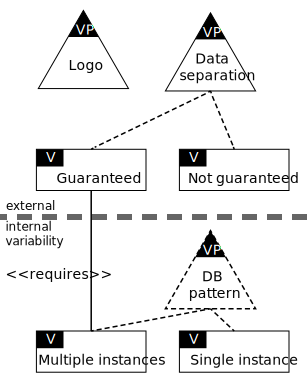
\includegraphics[width=0.48\textwidth]{assets/OVM}
    \caption{Example of a Variability Model in OVM notation}
    \label{fig:ovm}
\end{figure}

In OVM, the \textit{variation points} are the key items. One variation point has multiple \textit{variants} that are either optional or mandatory. Relations between VP's exist that define whether some variant is mutual exclusive with some other variant or whether some variant requires an other variant. Relations are drawn as lines between VP's. An example can be seen in figure \ref{fig:ovm}.

\subsubsection{Developing with variability in mind}
% Efficient customization of multi-tenant Software-as-a-Service applications with service lines
% by Stefan Walravena, Dimitri Van Landuyta, Eddy Truyena, Koen Handekynb, Wouter Joosena

\subsubsection{Variability Realization Techniques}
Jansen et al. \cite{jansen2010customization} note that while lot of research has been done on variability modeling, there is lack of research on techniques needed to implement variability. They identify five realization techniques of two types of customization, being \textit{Model View Controller (MVC) customization} and \textit{system customization}:
\begin{itemize}
\item \textbf{Model changes} allow tenants to fit the application to their domain. Model changes include changing entity attributes, adding entities and entity-relationships. Some changes require a more abstract application and therefore need to be thought upon earlier in the design process than more simple changes which could easily be added later on.
\item Some of the simpler customizations include \textbf{view changes} as in MVC patterns views don't interact with other components, but instead are the receiving part.
\item There is much freedom in \textbf{controller changes}, ranging from restricting data to one tenant only till fully customized workflows.
\end{itemize}
Large systems build of components delivering services can create variations of a different magnitude, on system level:
\begin{itemize}
\item \textbf{System connector changes} occur when connections to remote services are made variable. Examples include having multiple connectors for printing photos or multiple physical mail delivery providers.
\item With \textbf{system component changes} multiple components deliver the same service and are selected based on configuration.
\end{itemize}

Kabbedijk and Jansen \cite{kabbedijk2011variability} describe three variability realization techniques they observed in case studies. 
\textbf{Customizable Data Views} are a pattern to store tenant specific representation settings, eg. how tenants want to filter or sort their data. 
Although this technique also requires some table storing data and needs a small controller, it can be seen as mainly a view change as described by Jansen et al. 
Another view change is the \textbf{Module Dependent Menu}-pattern, to create menus that are dependent on the modules associated to a tenant. The last technique they observe is more a controller change. 
\textbf{Pre/Post Update Hooks} is a pattern to execute pieces of code before or after certain events happen in the application. 
This allows for tenants to enable or disable modules that check data or automate certain tasks.

Truyen et al. \cite{truyen2012context} introduce \textit{Context Oriented Programming (COP)} to implement what can be seen as controller changes. 
In COP layers are added to the code that override certain behavior when this layer is activated for a specific tenant. 
The overriding methods can still call the original method allowing them to modify the output or implement a filter. 
Multiple layers can be active at once, doing their work in a predefined order. 
% MAYBE-TODO: this paragraph could be more elaborate

Another common variation technique is \textit{dependency injection (DI)} \cite{walraven2011middleware} where one of the classes that implement an interface are injected by a provider. 
Walraven et al. mention in their Related Work section that Aspect Oriented Programming (another name for COP) proves more flexible in that way. 
In DI, no two 'modules' providing the same functionality can interact or extend each other, while in COP those implementations can work together. 
% MAYBE-TODO: this paragraph could be more elaborate

\subsubsection{future work in variability}
